%% 
%% Copyright 2007-2024 Elsevier Ltd
%% 
%% This file is part of the 'Elsarticle Bundle'.
%% ---------------------------------------------
%% 
%% It may be distributed under the conditions of the LaTeX Project Public
%% License, either version 1.3 of this license or (at your option) any
%% later version.  The latest version of this license is in
%%    http://www.latex-project.org/lppl.txt
%% and version 1.3 or later is part of all distributions of LaTeX
%% version 1999/12/01 or later.
%% 
%% The list of all files belonging to the 'Elsarticle Bundle' is
%% given in the file `manifest.txt'.
%% 
%% Template article for Elsevier's document class `elsarticle'
%% with numbered style bibliographic references
%% SP 2008/03/01
%% $Id: elsarticle-template-num.tex 249 2024-04-06 10:51:24Z rishi $
%%
%\documentclass[preprint,12pt]{elsarticle}
\documentclass[5p]{elsarticle}

%% Use the option review to obtain double line spacing
%% \documentclass[authoryear,preprint,review,12pt]{elsarticle}

%% Use the options 1p,twocolumn; 3p; 3p,twocolumn; 5p; or 5p,twocolumn
%% for a journal layout:
%% \documentclass[final,1p,times]{elsarticle}
%% \documentclass[final,1p,times,twocolumn]{elsarticle}
%% \documentclass[final,3p,times]{elsarticle}
%% \documentclass[final,3p,times,twocolumn]{elsarticle}
%% \documentclass[final,5p,times]{elsarticle}
%% \documentclass[final,5p,times,twocolumn]{elsarticle}

%% For including figures, graphicx.sty has been loaded in
%% elsarticle.cls. If you prefer to use the old commands
%% please give \usepackage{epsfig}

%% The amssymb package provides various useful mathematical symbols
\usepackage{amssymb}
%% The amsmath package provides various useful equation environments.
\usepackage{amsmath}
%% The amsthm package provides extended theorem environments
%% \usepackage{amsthm}

%% The lineno packages adds line numbers. Start line numbering with
%% \begin{linenumbers}, end it with \end{linenumbers}. Or switch it on
%% for the whole article with \linenumbers.
%% \usepackage{lineno}

% Own Packages
\usepackage{float}
\usepackage{nomencl}
\makenomenclature
% Take nomenclature title from a section named Glossary to conform to Elsevier guidance for authors
\renewcommand{\nomname}{\vspace{-.25in}}

\journal{Fusion Engineering and Design}

\begin{document}

\begin{frontmatter}

%% Title, authors and addresses

%% use the tnoteref command within \title for footnotes;
%% use the tnotetext command for theassociated footnote;
%% use the fnref command within \author or \affiliation for footnotes;
%% use the fntext command for theassociated footnote;
%% use the corref command within \author for corresponding author footnotes;
%% use the cortext command for theassociated footnote;
%% use the ead command for the email address,
%% and the form \ead[url] for the home page:
%% \title{Title\tnoteref{label1}}
%% \tnotetext[label1]{}
%% \author{Name\corref{cor1}\fnref{label2}}
%% \ead{email address}
%% \ead[url]{home page}
%% \fntext[label2]{}
%% \cortext[cor1]{}
%% \affiliation{organization={},
%%             addressline={},
%%             city={},
%%             postcode={},
%%             state={},
%%             country={}}
%% \fntext[label3]{}

\title{JET Plasma Control System Upgrade using MARTe2}

%% use optional labels to link authors explicitly to addresses:
%% \author[label1,label2]{}
%% \affiliation[label1]{organization={},
%%             addressline={},
%%             city={},
%%             postcode={},
%%             state={},
%%             country={}}
%%
%% \affiliation[label2]{organization={},
%%             addressline={},
%%             city={},
%%             postcode={},
%%             state={},
%%             country={}}

\author{A.V.~Stephen} %% Author name

%% Author affiliation
\affiliation{organization={Computing Division, United Kingdom Atomic Energy Authority},%Department and Organization
            addressline={Culham Campus}, 
            city={Abingdon},
            postcode={OX14 3DB}, 
            state={Oxfordshire},
            country={United Kingdom}}

%% Abstract
\begin{abstract}
%% Text of abstract

JET real-time plasma control has been delivered with a heterogeneous collection of control systems linked by a dedicated low-jitter, low-latency network. To provide a high degree of flexibility in tuning plasma control algorithms to experimental requirements, the Real-Time Central Controller (RTCC) has been available since 1997. RTCC provides a sandboxed execution environment where experimental algorithms can be deployed with a rapid development workflow. New control laws can be developed by operators during the course of an experimental session. The potential impact of a defect in algorithms evolved without full lifecycle quality assurance can be bounded by clipping feedback control requests at the actuator managers. The likelihood of such defects is reduced in the first place by constraining the algorithms to be composed from reusable blocks and trusted real-time signals. Although this system operated successfully for a long time, limitations in compute capacity of the legacy hardware on which the application was deployed constrained algorithm development.

Motivated by the need to provide physics operators with a more performant system, an upgrade project was carried out to port the RTCC application to a modern high performance PC platform. The architecture selected was to use the MARTe2 framework. Development was able to reuse existing MARTe2 data sources to connect the application to the JET environment using the ITER SDN protocol. RTCC blocks were converted to MARTe2 functions. Python tooling was created to automatically convert previously deployed RTCC algorithms to MARTe2 configuration form.

This paper describes the techniques used to demonstrate system correctness prior to deployment in the JET operating environment. This was particularly important given that it was deployed around the time of the DT campaigns. It explains how the system was used to demonstrate some novel control methods which delivered useful experiments in the final JET campaigns. It also outlines how the JET legacy data combined with this MARTe2 application can offer future value, even in the absence of the JET machine itself.
\end{abstract}

%%Graphical abstract
%% TODO: This is recommended
%\begin{graphicalabstract}
%\includegraphics{grabs}
%\end{graphicalabstract}

%% TODO: This is recommended
%%Research highlights
%%\begin{highlights}
%\item Research highlight 1
%\item Research highlight 2
%\end{highlights}

%% Keywords
\begin{keyword}
%% keywords here, in the form: keyword \sep keyword
real-time \sep control \sep MARTe2 \sep JET \sep QA

%% PACS codes here, in the form: \PACS code \sep code

%% MSC codes here, in the form: \MSC code \sep code
%% or \MSC[2008] code \sep code (2000 is the default)

\end{keyword}

\end{frontmatter}

%% Add \usepackage{lineno} before \begin{document} and uncomment 
%% following line to enable line numbers
%% \linenumbers

%% main text
%%

%% Use \section commands to start a section
\section{Introduction}
\label{sec:intro}
%% Labels are used to cross-reference an item using \ref command.

%\subsection{Background}

Plasma Control Systems\footnote{PCS - Plasma Control System} are large and complex.
There are variations in approach, but most fusion projects distinguish between
the disciplines of physics design and real-time system implementation.

Physics design is informed by, but usually separate from, first principles 
high-fidelity simulation. It works with macroscopic plasma quantities
and involves reduced order models with sufficient simplification to admit
practical use in a real-time environment.  This discipline combines
physics understanding of the main plasma and machine processes, along
with engineering control theory. Development typically uses modelling 
environments and may make use of experimental or synthetic data.

Real-time system implementation is tasked with converting the physics design
into a robust and resilient deterministic control system.  It must reproduce
the expected behaviour from the design system, in the real-world environment.
One challenge is to prove that the algorithm outcomes do not diverge from
the predicted path when running on different hardware, implemented in different
languages and frameworks. The performance of the code (in all possible paths) 
must be shown to be compatible with the dynamics time scales.  Delay is an enemy of 
control, time jitter effectively injects noise into a process.
The code must be free of race conditions, memory or other resource leaks
and defects.  If generated by tools, then those tools must be verified.
If generated by manual coding, adequate unit and integration tests must
be performed. 

In both cases, it is necessary to provide tooling and processes which support
evolution of the design, and the implementation.  This means tracking versions,
configuration, input data sets experienced by the codes, and the results and
verification of the correctness of these.  The lifecycle must also define
for how to iterate, when to migrate new features from design to implementation,
and how to commission and deploy.

Finally, management of off-normal events (often termed {\em exceptions}) 
must be addressed.  From the design point of view, exceptions include both
failure of the design to achieve control of the process dynamics (error of method)
as well as failure of equipment which prevents control (error of measurement or actuator).
Mitigations defined in the design must be implemented in real-time.  In addition
the real-time system must be able to degrade gracefully in the event of internal
exceptions (hardware faults or system corruption).

One of the design strategies for the JET plasma control system was to include
a flexible real-time central controller (RTCC). This was capable of 
addressing both engineering aspects directly, for a subset of the overall
design space.  This enabled very rapid prototyping of new control
algorithms during the course of JET experimental sessions.

This paper describes why it was necessary to upgrade JET RTCC as part of the
final JET operations campaigns.  It describes how the JET design principles
and system architectures reduced the risk and cost of this project to a 
level that made if feasible.  It describes the outcomes of the project, 
including the additional benefits that the work leaves for the future
exploitation of the JET data.


%The former abstracts higher level descriptions of the plasma control processes
%from the physics perspective. Thus dealing with magnetic, kinetic, MHD and error field
%control as well as wall conditioning, disruption and runaway electron control.
%Real-time system implementation must then map the control tasks into robust, resilient,
%deterministic control software. The implementation must deal with practical real-world
%constraints. These include signal processing to compute the required algorithm
%inputs, management of target control references throughout the shot, and provision 
%of exceptional handling strategies to resolve off-normal conditions (whether in the plasma,
%or in the sensor and actuator subsystems).

% TODO\cite
% https://www.sciencedirect.com/science/article/abs/pii/S0920379614000647
% Physics of the conceptual design of the ITER plasma control system 
%
%
% NO IT DOESN'T : IT DESCRIBES ONE UPGRADE WHICH TACKLED BOTH-ish

%This paper concentrates on the second challenge, of real-time plasma control system implementation.

%The order of the paper is $\ldots$ % TODO



% RENAME Materials and Methods, but that is the spirit
\section{Infrastructure and Architecture}

\subsection{JET PCS Infrastructure}
\label{l_infrastructure}

The JET PCS infrastructure was
distributed} and heterogeneous\footnote{JET has entered decommissioning, and although the PCS systems still exist, they no longer operate}.  
It was divided into around 80 subsystems spanning measurement, control, and protection functions.
This separation was required partly for organisational reasons: to divide the responsibility, and the work.
It was also beneficial to achieve sufficient decoupling to permit evolution without excessive risk.

The variability in technologies in implementation arose partly from differences in
optimal design choices and constraints across the project.  It was also enforced
as the project lifetime extended and as generations of software and hardware
evolved through industry cycles.

Where collections of subsystems were required to work collectively, real-time data was
shared as required. As one example, magnetics sensor data was acquired by the KC1D
diagnostic, and provided to the plasma shape and position controller.  During early
phases of the project, these real-time links were dedicated point to point connections.
The infrastructure became more fully connected with the introduction of a comprehensive
real-time data network.  This was initially implemented using Asynchronous Transfer Mode (ATM)
telecomms technology (effective, but highly bespoke). A later upgrade extended the
real-time network using standard ethernet equipment, and adopting the ITER Synchronous Databus
Network (SDN) protocol.


\subsection{JET PCS Architecture}
\label{l_architecture}

The JET PCS architecture is shown in figure~\ref{fig:pcs}. 
It comprises four main groups: measurements, local feedback, global feedback and actuators.
The arrows indicate information flows, including pre-configured parameter values, and
real-time data.  Some of the core functions operate mostly within the inner local feedback
loop.  This includes the main magnetic, heating and fuelling loops.  More sophisticated
control, and protection, are provided through the real-time central controller (RTCC) 
and auxiliary real-time signal server (RTSS).

Each of the individual systems may be implemented using a variety of technology.
The unifying aspects of the architecture are a standard real-time data exchange
protocol\cite{Felton}, and a common parameter management system (Level-1\cite{Farthing}).


\begin{figure}[ht!]
\centering
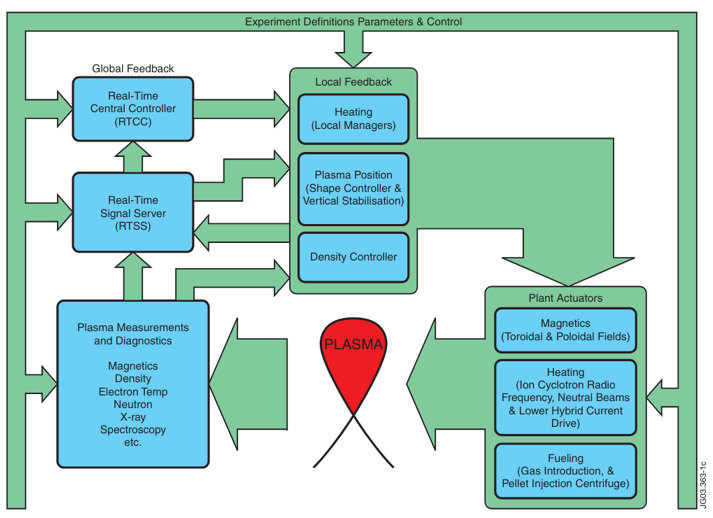
\includegraphics[width=0.5\textwidth]{JG_Felton.PNG}
	\caption{The JET Plasma Control System (PCS) architecture.  \cite{Felton99}}
\label{fig:pcs}
\end{figure}

\subsection{JET Real-Time Central Controller}
\label{s_rtcc}

The function of the standard local control systems was to establish 
common plasma operating states (scenarios), mostly based on 
pre-calculated feed-forward references (with feedback control to stabilise
around particular operating points).  As such, these control systems
had a stable development lifecycle, with modifications and enhancements
generally being implemented during long shutdown periods.

To provide more advanced control, of plasma parameters for which the
relationship between direct measurement and fixed actuator response, 
it was necessary to add a more flexible and dynamic controller.
This real-time central controller (RTCC) provided a library of
reusable calculation blocks.  Using a custom editor, the physics
operator was permitted to design a control algorithm as a 
sequential graph (or {\em network}) of up to 200 blocks.
Up to four concurrent RTCC networks could be executed.

Figure~\ref{fig:tf} shows the documentation for one of these calculation
blocks (a first order transfer function). Each block received a variable
number of analogue inputs (continuously varying signals) as well as
one digital input. Blocks to express logical combinations, as well as
signal transformation were provided.  
The RTCC networks could therefore encompass 
control flow as well as signal processing.

Provision was made for all of the
usual mathematical operators, as well as for higher level functions such
as waveform generation, and PID control.  One limitation was that
only scalar valued signals could be treated.  Vector oriented control
schemes were possible, but had to be expressed as sets of scalar 
expressions.

\begin{figure}[ht!]%% placement specifier
\centering
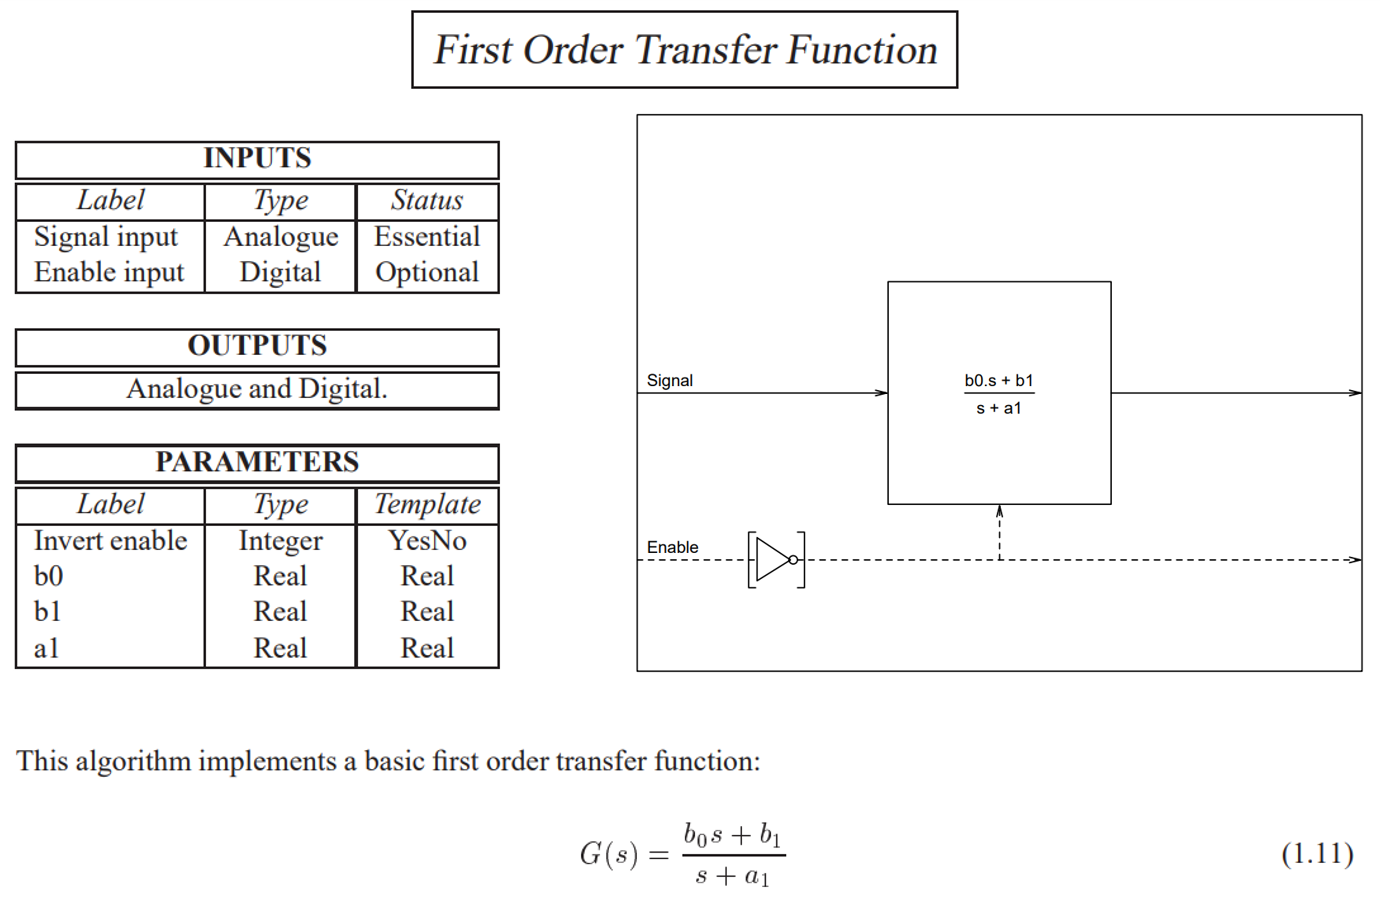
\includegraphics[width=0.5\textwidth]{RTCC_TF1_BLOCK.PNG}
\caption{The first order transfer function block. One of approximately 40 reusable components
	available for physics operators to design control schemes on-the-fly in RTCC.}
\label{fig:tf}
\end{figure}

Using this toolkit, a specialist operator---the Plasma Duty Officer (PDO)
would take instruction from the Session Leader (SL) as to the required
control schemes needed to support an experimental session.
The PDO team built an extensive library of RTCC networks.
Typical responsibilities for the PDO could be to modify the
networks to probe and tune gains, to replace diagnostic
signals by alternatives or to develop entirely new schemes.

The software tools to support the role were sufficient, but
required training and had some idiosynchrasies and limitations.
Proposals to improve the applications were put forward, but
ease of use was not seen as a sufficiently high priority to
allocate resources.  Figure~\ref{fig:editor} shows the tabular
graph editor. Each row on the left instantiates one of the 
blocks, and the output is assigned to the identifier on the right.
While a supporting viewer which could render the defined network
as a graph was available, the graphical view did not support
editing.

\begin{figure}[ht!]%% placement specifier
\centering
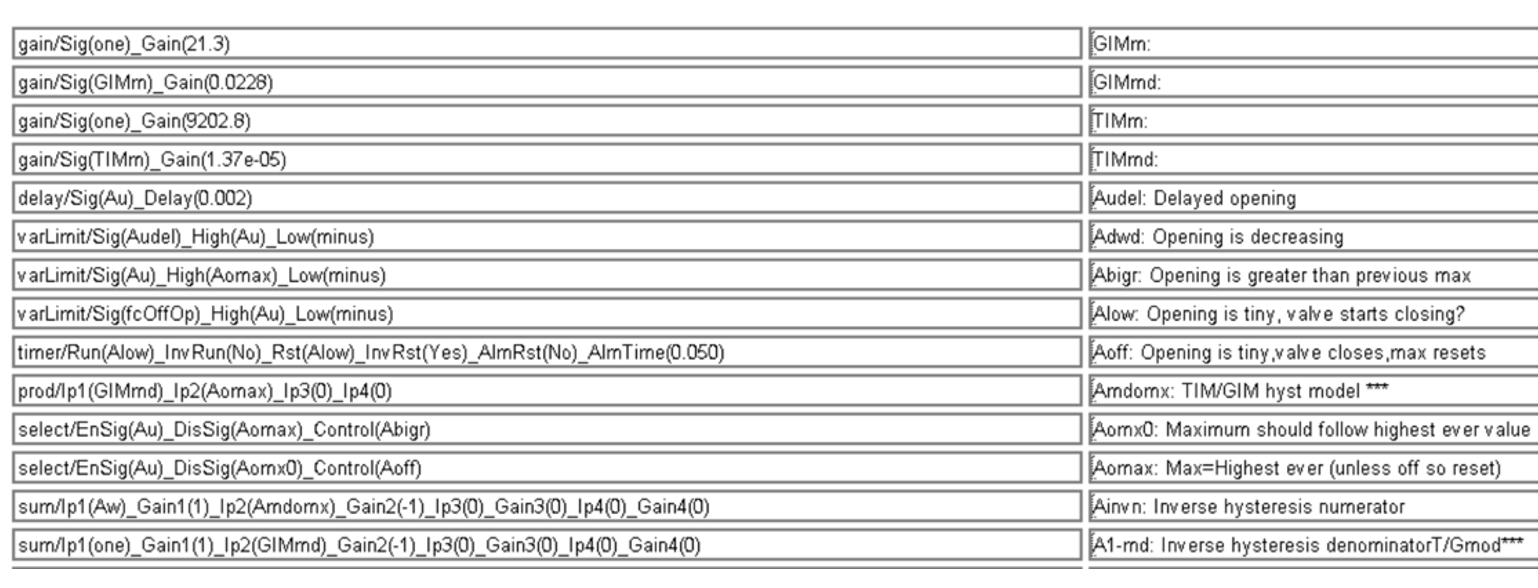
\includegraphics[width=0.5\textwidth]{L1RTCC.PNG}
\caption{The tabular RTCC network editor, implemented in JET Level-1 software.}\label{fig:editor}
\end{figure}


%Termed the {\em real-time central controller (RTCC)} this system was
%part of a suite of general real-time services targeting advanced
%real-time control research.  The RTCC system was an application 
%capable of receiving a very wide (and variable) set of input signals
%aggregated and managed by a companion system, the {\em real-time signal server (RTSS)}.
%
%The architecture of this RTCC application was the common pattern of
%a real-time execution engine configurable with a graph of signal
%processing blocks.  The library of blocks supported signal ingress,
%filtering and validation to achieve estimates of plasma parameter
%state.  Entities to implement control schemes, such as a proportional/integral/derivative
%(PID controller), transfer functions and general calculation support
%could then be combined to explore control concepts.  An option to
%use real-time computed references for the actuator systems, and to 
%use these in place of the nominal feedfoward time series was also
%provided.

The outputs from RTCC networks could be routed to the actuator systems
to provide references overriding the pre-configured local control.
In view of the flexibility, control systems generally offered a restricted
window within which demands would be accepted.
Some RTCC networks were also allocated to computing protection signals,
and could be used to trigger protective actions if limits were breached.

Following the major ITER-like wall project in 2011, the original RTCC
system was duplicated so that one instance be dedicated to running
protection networks, while the other was used for experimental functions.
This reduced the likelihood that a protection network be misconfigured.

\subsubsection{RTCC Limitations}

As JET enhancements delivered ever more real-time diagnostic signals,
and expanded the capability of the control systems, the demands
on the RTCC system increased.  Larger networks, consuming more data,
required more CPU and memory, or risked skipping control cycles
and losing information.

An upgrade to RTCC was required to be able to support the needs
of the JET TaskForce planned experiments.  Planning the design, implement,
testing and commissioning of the upgrade required considerable
care given the criticality of the system to oeprations.


\subsubsection{Upgrade Project Requirements and Constraints}

The minimum project requirements were to 
upgrade the system so as to deliver the following.

\begin{itemize}
	\item[REQ-1]{The required increased capacity in processing and storage.}
	\item[REQ-2]{Full backwards compatibility to reuse any previous control scheme.}
	\item[REQ-3]{Minimised risk to operations}
\end{itemize}

The project team were encouraged to find a design solution which
if possible would in addition

\begin{enumerate}
	\item[REQ-4]{Support rapid development of new components.}
	\item[REQ-5]{Improve the physics user experience.}
\end{enumerate}

The original implementation assumed a particular hardware platform
and operating system.  It was also written as a single, large
C application.  The configuration of the data structures was
complex and relied on automatically generated intermediate
files through scripts developed with legacy tools. 

\section{Methodology and Design Approach}

% FIGURE? JG03.363-1c ? The Felton diagram.

%% TOCITE Level-1 paper ?

Overall coordination and configuration of these disparate systems was achieved through coordinating systems, services
and applications.

\subsection{MARTe}

\begin{figure}[ht!]%% placement specifier
\centering
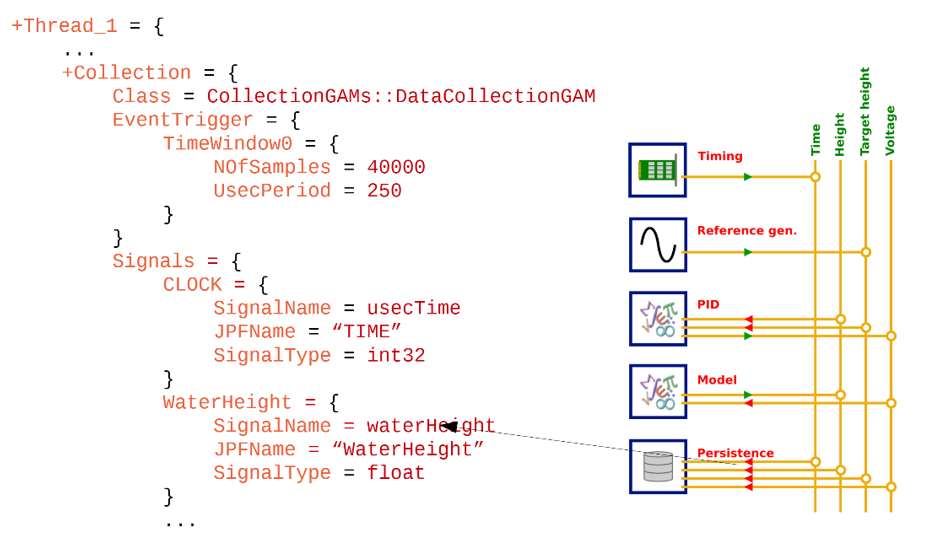
\includegraphics[width=0.5\textwidth]{MARTE.PNG}
%\vspace{1.5in}
\caption{MARTe}\label{fig4}
\end{figure}

\subsection{Software Frameworks}

Contemporaneously with this CFW development, the Plasma Operations Group had decided
to take a very structurally equivalent approach to building real-time control applications.
Their application, the now well known Multi-threaded Application for Real-Time execution (MARTe),
also consists in a run-time which instantiates objects from a structured configuration file.
Implemented in C++, and targeting high performance, low jitter, high reliability control
applications it also provided some measure of tooling for rapid application development.
To manage the aggregation and customisation of configuration files, MARTe at JET made
use of the Level-1 configuration tool to manage templates, parameter substitution and
code generation algorithms.

JET plasma control made significant use of the MARTe system, implementing key systems
including shape control, vertical stabilisation, walls (estimating the energy load on the first wall),
EFCC control, vessel-thermal map and the ILW real-time protection sequencer.  These applications
were in use from the early 2000s and were fully integrated with the other JET operations software
(configuration, monitoring, data acquisition and the RTDN ATM network).

Around 2014, at F4E, following failed attempts to find a comparable COTS software system 
on the market, a project to harden MARTe to a level suitable for deployment at ITER 
was undertaken.  The outcome of this work was MARTe2.  In addition to code review and improvement,


\subsection{Real-Time Data Network}

The second unifying service was the real-time data network. This was a high performance, dedicated private network with low latency and low jitter communications between all of the PCS systems.  The communications topology was point to multi-point. Implementation translated across three generations of networking equipment.  The early version of the network ran over 100Mbps ethernet using UDP unicast. An upgrade in the mid 1990s introduced telecommunication standard equipment using ATM\footnote{} switches in which the delivery of data was configured in the switch. In 2016, motivated by the increasing difficulty in obtaining ATM equipment, the ITER SDN ethernet multicast solution was adopted.

\subsection{Configuration Management}

  Most importantly, the {\em Level-1} configuration management subsystem provided a consistent and detailed model of each subsystem. Representing the attributes and modifiable options for each subsystem as rich parameters, the {\em Level-1} database, user interfaces, and codes provided a meta-programming system for the overall PCS.  This configuration tooling was
used to define all of the control settings to achieve a given experimental goal (parameter values, calibration, reference time series and inter-system dependencies).  This system tuning was required to be completed before a JET discharge could begin.  


\section{Upgrade Outcomes and Benefits}

%GUI RTCC Block Library

%\begin{figure}[t]%% placement specifier
%\centering
%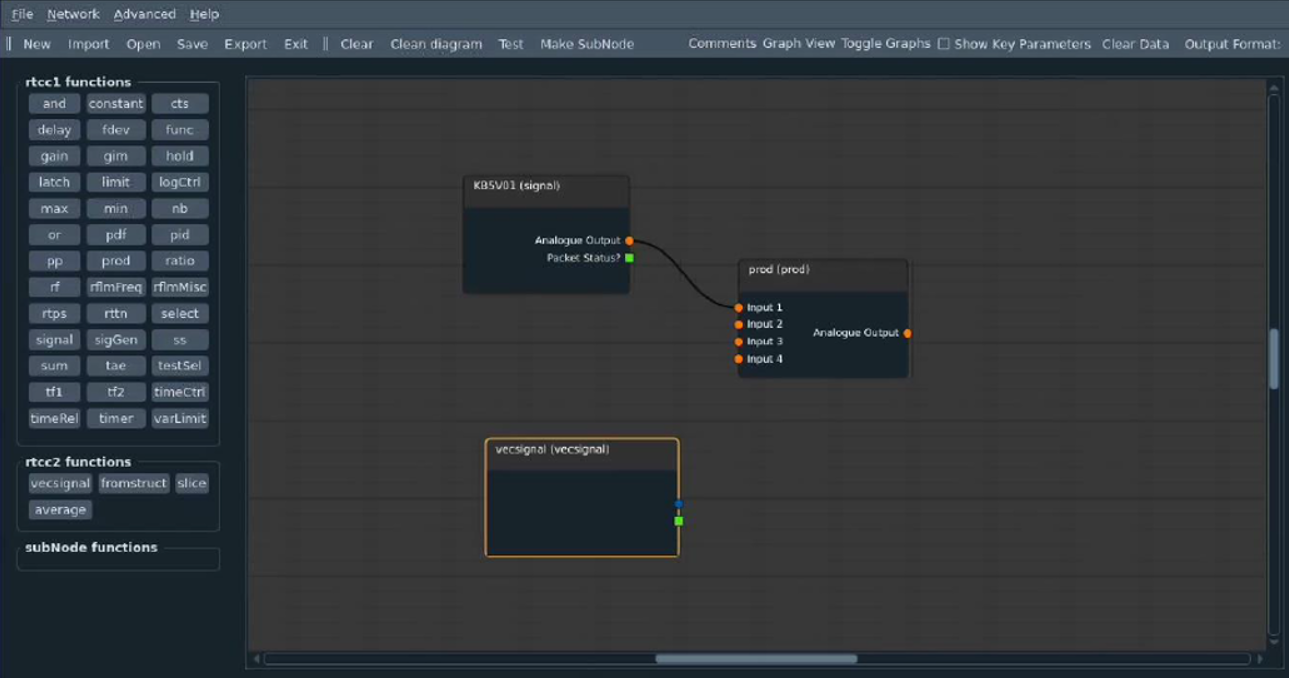
\includegraphics[width=0.5\textwidth]{GUI.PNG}
%\caption{RTCC Block Library}
%\label{fig6}
%\end{figure}

Each of the calculation blocks in the RTCC application were ported to MARTe2 {\em Functions}.
Atypically, the standard block template consisted in a combined vector of value and status.
This protocol was retained in the updated implementation. This was important to simplify
translating algorithm definitions from the original notation to MARTe2 format.

The outline structure of the RTCC2 MARTe2 application was istraightforward.
High level service declarations common to most JET MARTe applications
instantiated an introspection service, a pulse oriented state machine, 
and the main data flow superstructure.

Python translation support modules handled the translation of RTCC network 
descriptions into MARTe2 configuration syntax, using the new {\em Functions}.
In addition to generating the {\em Function} instances (a simple 1:1 mapping),
the translation also created auxiliary objects to manage automatic
recording of computed values.  Managing automatic name generation is one
of the main tasks in this process.  This introduces a design question.  From
the perspective of efficiency, and to simplify the translation code, 
auto-generated names which lack comprehensibility are a good choice. 

This leaves code review in the domain of the meta-programming code, 
which is practical for checking the intent.  The disadvantage of this
approach however is that if the detailed results from executing the 
algorithms differ from expected values, it is difficult to analyse
the intermediate signals as their relationship to the calculation is
masked by the anonymous names.


\begin{figure}[t!]%% placement specifier
\centering
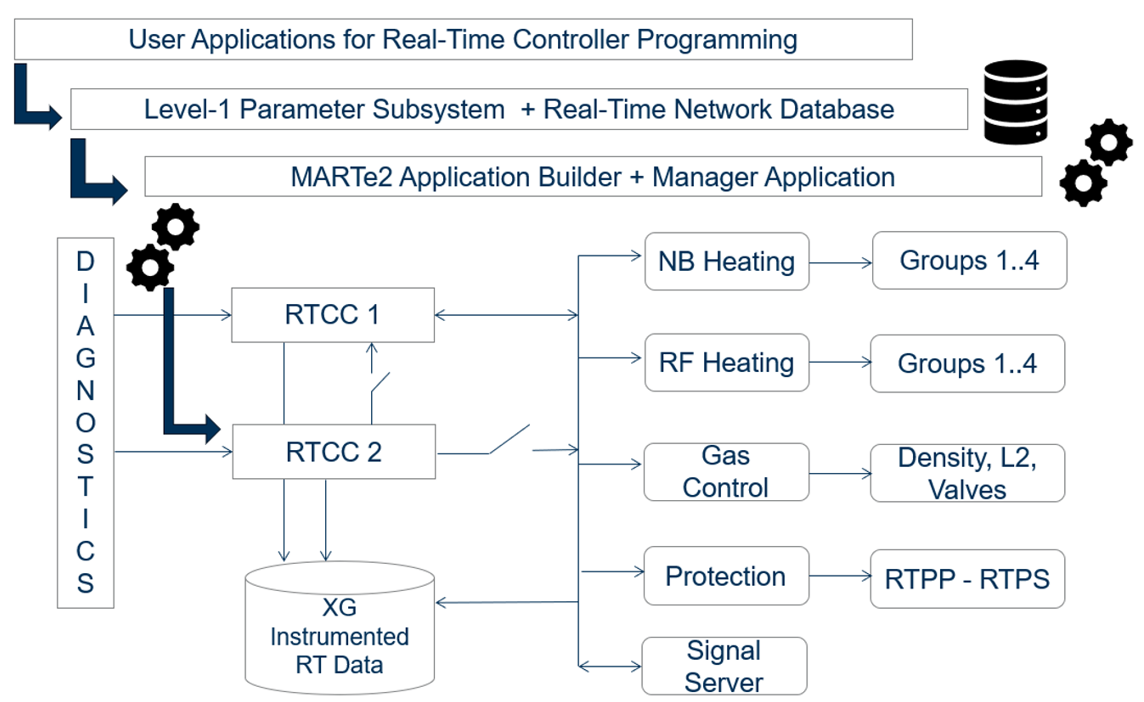
\includegraphics[width=0.5\textwidth]{R1R2ARCH.PNG}
%\vspace{1.5in}
\caption{RTCC Block Library}\label{fig5}
\end{figure}
\section{Discussion}

Best practice in both system engineering and software engineering 
aligns with the patterns applied in the design of the JET plasma control system.

From a system engineering perspective, it is highly desirable to be
able to trace functions to requirements and vice-versa. Computer
aided design tools to support this workflow are growing in capability.
The trend is towards model-based system engineering (MBSE).  Some
practitioners are integrating quantitative simulations within this
model space. This is generally a top-down engineering flow.

From a software engineering perspective, test based development seeks
to increase confidence in the correctness of software components.
Optimal quality can be achieved through the design and rigorous testing
of reusable modules.  Reusability through composition and configuration
is an effective technique to define scope boundaries for modules.
Integrated tests then bound the capability of component assemblies.
This is a generally bottom-up engineering flow.

Two approaches to bring the system engineering and software engineering
together are code generation, and domain specific language definition.
Indeed, they are complementary techniques, and create the possibility
of a three-tiered engineering stack.

From a computer science point of view, there is no theoretical difference
between high-level and low-level languages.  They are invariably
turing complete and hence equivalent. The question is then whether the
tools are effective in supporting subject matter experts and 
implementation engineers to meet system objectives.
Automated support for assuring quality can be applied at three
levels.

In terms of basic definition, automated tools for avoiding trivial errors of expression
are beneficial.  In low level languages, these are syntax checkers
and source code "linters".  Although not named equivalent, model
based system engineering tools provide similar support to assure
structural and lexical consistency.

Where components are combined to applications,
static analyzers can apply more sophisticated logic to
be able to reason about the semantics of the representation
of the system.  In the system engineering space, compliance 
matrices verify completeness.  In the software engineering
space, verifying type consistency is one of many examples
of automatically identifying errors of reasoning.

Both of these techniques can be applied to the model/code
by analysis of the structural representation.

When executed, dynamic semantic checking can analyse the 
correctness of the system by tracking function call
patterns and data flows.

For a given stack of system models, 
software frameworks, and tooling or manual procedure which
can map across the semantic space, there are three
measures of effectiveness.

Firstly - whether the mid-level tooling - code generators and/or formal
DSLs are supported by intelligent IDEs.  Support can range from none,
through in-house development of plugins for existing IDEs and all the
way to systems such as the proprietary MPS system.

Secondly - whether the three levels and the integration flows
between them are complete and sufficient to fully describe
the system.  The law of diminishing returns and pareto principle
can encourage projects to accept that it is not economically
feasible for the end to end design flow to achieve 100\%
coverage.

Finally, there are impedance mismatches between subject matter experts
across these three levels of formal design activity.  Each formalism
(system engineering, domain specific language engineering, software
engineering) has a skillset, methodology and jargon.  The relationships
between the problem domain and each of these disciplines are complex.
The solution space is broad. Ultimately, as with mathematical proof,
the overall success of a design depends on how well the team has
communicated.

This pattern is well understood by software engineers.  As problems
become larger and more complex, it becomes necessary to invent
abstractions and internal tools to make engineering tractable.
The expectation is that the return on investment on these jigs
and supporting skeletons will come when requirements shift.
One risk is that the complexity of the newly minted supports,
which can be unique to the project, create a skill risk.
The other is that the shift in the requirements breaks
assumptions upon which the support tools depended.  This 
can inevitably be fixed, at the cost of entropy and
"technical debt".  

Mathematically, the extrema of these trade-offs is captured
in Godel's theorem.  We can have a system in which all statements
can be proved, but such systems are extremely limited in the
range of behaviours they can model.  A system that has the capacity
to model the complexity we need in practice necessarily 
contains unprovable statements.



Granularity, reuse and code generation.

The question of how to preserve human readability of generated code...

\subsection{Engineering Approaches}

\begin{itemize}
\item{Monolithic}
\item{Distributed}
\item{MBSE}
\item{Custom Code}
\item{Frameworks}
\item{Integration Ecosystems}
\end{itemize}

\subsubsection{Domain Specific Languages (DSLs)}

Where data driven applications achieve a certain level of reconfiguration, they are more commonly
described in computer science as {\em domain specific languages (DSLs)}. DSLs are characterised
as a programming language designed for a specific use case.  Benefits of DSLs are that they 
offer a higher level of abstraction optimized for a specific class of problem. Two classes
of domain specific language are typically identified. {\em External} DSLs separate the DSL
code from the standard code (written in a general programming language).  {\em Internal} DSLs
mix the DSL code and the general-purpose code in the same file.  This is general achieved by
embedding the DSL into the general-purpose code as a set of libraries or extensions.

In both cases, there is a challenge to adequately support the new task of programming
in the invented language.  To be effective, general purpose programming languages must
formally define syntax and semantics. They must be supplied with compilers, or interpreters.
These language tools are expected to be extended with support for trapping and explaining
syntax errors as a minimum, and semantic errors preferably.  To increase productivity, 
engineers working in a language also expect more advanced features such as code completion
and automated documentation.

For external DSLs, providing language support for basic control flow and iteration
can help to make programs more efficient and comprehensible.  A common design pattern
to deliver this support is to use code templating and code generation.  This
{\em meta-programming} increases productivity, but at the cost of adding another
layer of complexity in the tool stack.



\section{Conclusion}

% Comments on DSLs and tooling.
The RTCC system enabled JET real-time control experiments to adapt rapidly to new information
and ideas because the round trip time from concept to implementation did not require 
external software engineering. This was made possible by offering a flexible, but 
constrained programmable environment.

The project to upgrade RTCC 
successfully delivered the minimum project goals of increased capacity with
full backwards compatibility to reuse all previous control scheme definitions.
This was done without loss of operational time.
In addition, the stretch goals of increasing capability and improving
usability for end users were addressed.  

This change to a critical part of the JET plasma control system, implemented
at one of the most sensitive times in the programme life was enabled by 
sound historical architecture choices. These were both based on abstracting
the definition of real-time data flow and processing into machine 
processable formats. In respect of inter-system communication, this was the
real-time data network database, implemented using CODAS Configuration Language
(CCL) with automatic code generation.  In respect of intra-system algorithm
representation, this was via the RTCC network graph, and the equivalent RTCC2
object graph.  

The project feasibility rested not solely on these architectural patterns,
but on the MARTe framework and the improvements
and extensions made to this software in preparation for ITER.  
The JET real-time network extension to ethernet and use of SDN in 2016
provided a solid foundation.  The quality assurance and functional updates delivered
by the F4E MARTe2 project reduced the RTCC upgrade risk to an acceptable level.


The JET real-time algorithm executor has been ported to a future-proof and future-relevant framework.
The implementation leaves the possibility to rerun former JET shots against a virtualised
version of RTCC2. This opens the possibility to running virtual JET experiments.
These can test alternative state estimation concepts just by replaying the historic data.
By replacing dynamic elements with models, a closed loop virtual JET emulator could be demonstrated.
This could have a number of valuable use cases.

\newpage

Lorem ipsum
Lorem ipsum
Lorem ipsum
Lorem ipsum
Lorem ipsum
Lorem ipsum
Lorem ipsum
Lorem ipsum
Lorem ipsum
Lorem ipsum
Lorem ipsum
Lorem ipsum
Lorem ipsum
Lorem ipsum
Lorem ipsum
Lorem ipsum
Lorem ipsum
Lorem ipsum
Lorem ipsum
Lorem ipsum
Lorem ipsum
Lorem ipsum
Lorem ipsum
Lorem ipsum
Lorem ipsum
Lorem ipsum
Lorem ipsum
Lorem ipsum
Lorem ipsum
Lorem ipsum
Lorem ipsum
Lorem ipsum
Lorem ipsum
Lorem ipsum
Lorem ipsum
Lorem ipsum
Lorem ipsum
Lorem ipsum
Lorem ipsum
Lorem ipsum
Lorem ipsum
Lorem ipsum
Lorem ipsum
Lorem ipsum
Lorem ipsum
Lorem ipsum
Lorem ipsum
Lorem ipsum
Lorem ipsum
Lorem ipsum
Lorem ipsum
Lorem ipsum
Lorem ipsum
Lorem ipsum
Lorem ipsum
Lorem ipsum
Lorem ipsum
Lorem ipsum
Lorem ipsum
Lorem ipsum
Lorem ipsum
Lorem ipsum


%%\section{Glossary}
%%
%%
%%Field specific terms.
%%\begin{itemize}
%%\item[ATM]{Asynchronous Transmission Mode.  A low-latency telecommunications protocol standard.}
%%\item[DSL]{Domain Specific Language}
%%\item[MARTe]{Multi-threaded Application for Real-Time execution.  Software framework from JET.}
%%\item[MARTe2]{Enhanced version of MARTe developed by F4E for ITER.}
%%\item[Real-Time Thread]{The unit of concurrency in a MARTe2 application.}
%%\item[DataSource]{A service which abstracts device drivers to handle application I/O in a MARTe2 application.}
%%\item[Function]{The unit of compute in a MARTe2 application.  Each Real-Time Thread calls one or more Functions.}
%%\item[JET]{Joint European Tokamak}
%%\item[MBSE]{Model Based System Engineering}
%%\item[PCS]{Plasma Control System}
%%\item[RTCC]{Real-Time Central Controller.  A core application in the JET PCS.}
%%\item[SDN]{Synchronous Databus Network.  An ITER real-time network protocol.}
%%\item[UDP]{User Datagram Protocol. A connectionless data transport method in networking.}
%%\end{itemize}

\section{Gloassary}

\nomenclature{ATM}{Asynchronous}
\nomenclature{DSL}{Domain Specific Language}
\nomenclature{MARTe}{Multi-threaded Application for Real-Time execution.  Software framework from JET.}
\nomenclature{MARTe2}{Enhanced version of MARTe developed by F4E for ITER.}
\nomenclature{Real-Time Thread}{The unit of concurrency in a MARTe2 application.}
\nomenclature{DataSource}{A service which abstracts device drivers to handle application I/O in a MARTe2 application.}
\nomenclature{Function}{The unit of compute in a MARTe2 application.  Each Real-Time Thread calls one or more Functions.}
\nomenclature{JET}{Joint European Tokamak}
\nomenclature{MBSE}{Model Based System Engineering}
\nomenclature{PCS}{Plasma Control System}
\nomenclature{RTCC}{Real-Time Central Controller.  A core application in the JET PCS.}
\nomenclature{SDN}{Synchronous Databus Network.  An ITER real-time network protocol.}
\nomenclature{UDP}{User Datagram Protocol. A connectionless data transport method in networking.}

\printnomenclature

\section{Abbreviations}

Check that non-standard abbrevs are defined in a footnote on page 1.

\section{Acknowledgements}

Individuals who helped (but were not co-authors).

\section{Author Contributions}
Using CRediT taxonomy.

\begin{itemize}
\item[Conceptualization]{}
\item[Data Curation]{}
\item[Formal analysis ]{}
\item[Funding acquisition]{}
\item[Investigation]{}
\item[Methodology]{}
\item[Project administration]{}
\item[Resources]{}
\item[Software]{}
\item[Supervision]{}
\item[Validation]{}
\item[Visualization]{}
\item[Writing - draft]{}
\item[Writing - review and editing]{}
%% See https://www.elsevier.com/researcher/author/policies-and-guidelines/credit-author-statement
\end{itemize}

\section{Funding}

This work was supported by $ldots$
%% The Appendices part is started with the command \appendix;
%% appendix sections are then done as normal sections

\appendix
\section{Example Appendix Section}
\label{app1}

Appendix text.

%% For citations use: 
%%       \cite{<label>} ==> [1]

%%
Example citation, See \cite{lamport94}.

%% If you have bib database file and want bibtex to generate the
%% bibitems, please use
%%
%%  \bibliographystyle{elsarticle-num} 
%%  \bibliography{<your bibdatabase>}

%% else use the following coding to input the bibitems directly in the
%% TeX file.

%% Refer following link for more details about bibliography and citations.
%% https://en.wikibooks.org/wiki/LaTeX/Bibliography_Management

\begin{thebibliography}{00}

%% For numbered reference style
%% \bibitem{label}
%% Text of bibliographic item

\bibitem{lamport94}
  Leslie Lamport,
  \textit{\LaTeX: a document preparation system},
  Addison Wesley, Massachusetts,
  2nd edition,
  1994.

\end{thebibliography}
\end{document}

\endinput
%
%% Template Code follows


%% Use \subsection commands to start a subsection.
\subsection{Example Subsection}
\label{subsec1}

Subsection text.

%% Use \subsubsection, \paragraph, \subparagraph commands to 
%% start 3rd, 4th and 5th level sections.
%% Refer following link for more details.
%% https://en.wikibooks.org/wiki/LaTeX/Document_Structure#Sectioning_commands

\subsubsection{Mathematics}
%% Inline mathematics is tagged between $ symbols.
This is an example for the symbol $\alpha$ tagged as inline mathematics.

%% Displayed equations can be tagged using various environments. 
%% Single line equations can be tagged using the equation environment.
\begin{equation}
f(x) = (x+a)(x+b)
\end{equation}

%% Unnumbered equations are tagged using starred versions of the environment.
%% amsmath package needs to be loaded for the starred version of equation environment.
\begin{equation*}
f(x) = (x+a)(x+b)
\end{equation*}

%% align or eqnarray environments can be used for multi line equations.
%% & is used to mark alignment points in equations.
%% \\ is used to end a row in a multiline equation.
\begin{align}
 f(x) &= (x+a)(x+b) \\
      &= x^2 + (a+b)x + ab
\end{align}

\begin{eqnarray}
 f(x) &=& (x+a)(x+b) \nonumber\\ %% If equation numbering is not needed for a row use \nonumber.
      &=& x^2 + (a+b)x + ab
\end{eqnarray}

%% Unnumbered versions of align and eqnarray
\begin{align*}
 f(x) &= (x+a)(x+b) \\
      &= x^2 + (a+b)x + ab
\end{align*}

\begin{eqnarray*}
 f(x)&=& (x+a)(x+b) \\
     &=& x^2 + (a+b)x + ab
\end{eqnarray*}

%% Refer following link for more details.
%% https://en.wikibooks.org/wiki/LaTeX/Mathematics
%% https://en.wikibooks.org/wiki/LaTeX/Advanced_Mathematics

%% Use a table environment to create tables.
%% Refer following link for more details.
%% https://en.wikibooks.org/wiki/LaTeX/Tables
\begin{table}[t]%% placement specifier
%% Use tabular environment to tag the tabular data.
%% https://en.wikibooks.org/wiki/LaTeX/Tables#The_tabular_environment
\centering%% For centre alignment of tabular.
\begin{tabular}{l c r}%% Table column specifiers
%% Tabular cells are separated by &
  1 & 2 & 3 \\ %% A tabular row ends with \\
  4 & 5 & 6 \\
  7 & 8 & 9 \\
\end{tabular}
%% Use \caption command for table caption and label.
\caption{Table Caption}\label{fig1}
\end{table}


%% Use figure environment to create figures
%% Refer following link for more details.
%% https://en.wikibooks.org/wiki/LaTeX/Floats,_Figures_and_Captions
\begin{figure}[t]%% placement specifier
%% Use \includegraphics command to insert graphic files. Place graphics files in 
%% working directory.
\centering%% For centre alignment of image.
\includegraphics{example-image-a}
%% Use \caption command for figure caption and label.
\caption{Figure Caption}\label{fig1}
%% https://en.wikibooks.org/wiki/LaTeX/Importing_Graphics#Importing_external_graphics
\end{figure}


%% The Appendices part is started with the command \appendix;
%% appendix sections are then done as normal sections
\appendix
\section{Example Appendix Section}
\label{app1}

Appendix text.

%% For citations use: 
%%       \cite{<label>} ==> [1]

%%
Example citation, See \cite{lamport94}.

%% If you have bib database file and want bibtex to generate the
%% bibitems, please use
%%
%%  \bibliographystyle{elsarticle-num} 
%%  \bibliography{<your bibdatabase>}

%% else use the following coding to input the bibitems directly in the
%% TeX file.

%% Refer following link for more details about bibliography and citations.
%% https://en.wikibooks.org/wiki/LaTeX/Bibliography_Management

\begin{thebibliography}{00}

%% For numbered reference style
%% \bibitem{label}
%% Text of bibliographic item

\bibitem{lamport94}
  Leslie Lamport,
  \textit{\LaTeX: a document preparation system},
  Addison Wesley, Massachusetts,
  2nd edition,
  1994.

\end{thebibliography}
\end{document}

\endinput
%%
%% End of file `elsarticle-template-num.tex'.

